\subsection*{How is Generative Models Related to Japanese Anime?}

In the book chapter {\it Opening the Closed World of Shojo Manga (girl's comics)},
Takahashi argued that the doll-like saucer eyes of shojo girls is a representation
of the complex inner psychology of the girls \cite{takahashi2008shojo}.
Arguing against critics who think the eyes are unrealistic,
Takahashi stated that the ``enormous eyes with long eyelashes''
allows the audience to better engage to the plot emotionally.
However, since current generation of AI are based on statistical learning,
the images they generate are only based on training example.
That means the AI models will learn all the shojo unrealistic features
without expressing any inner emotion of the characters.
\begin{figure}[h]
    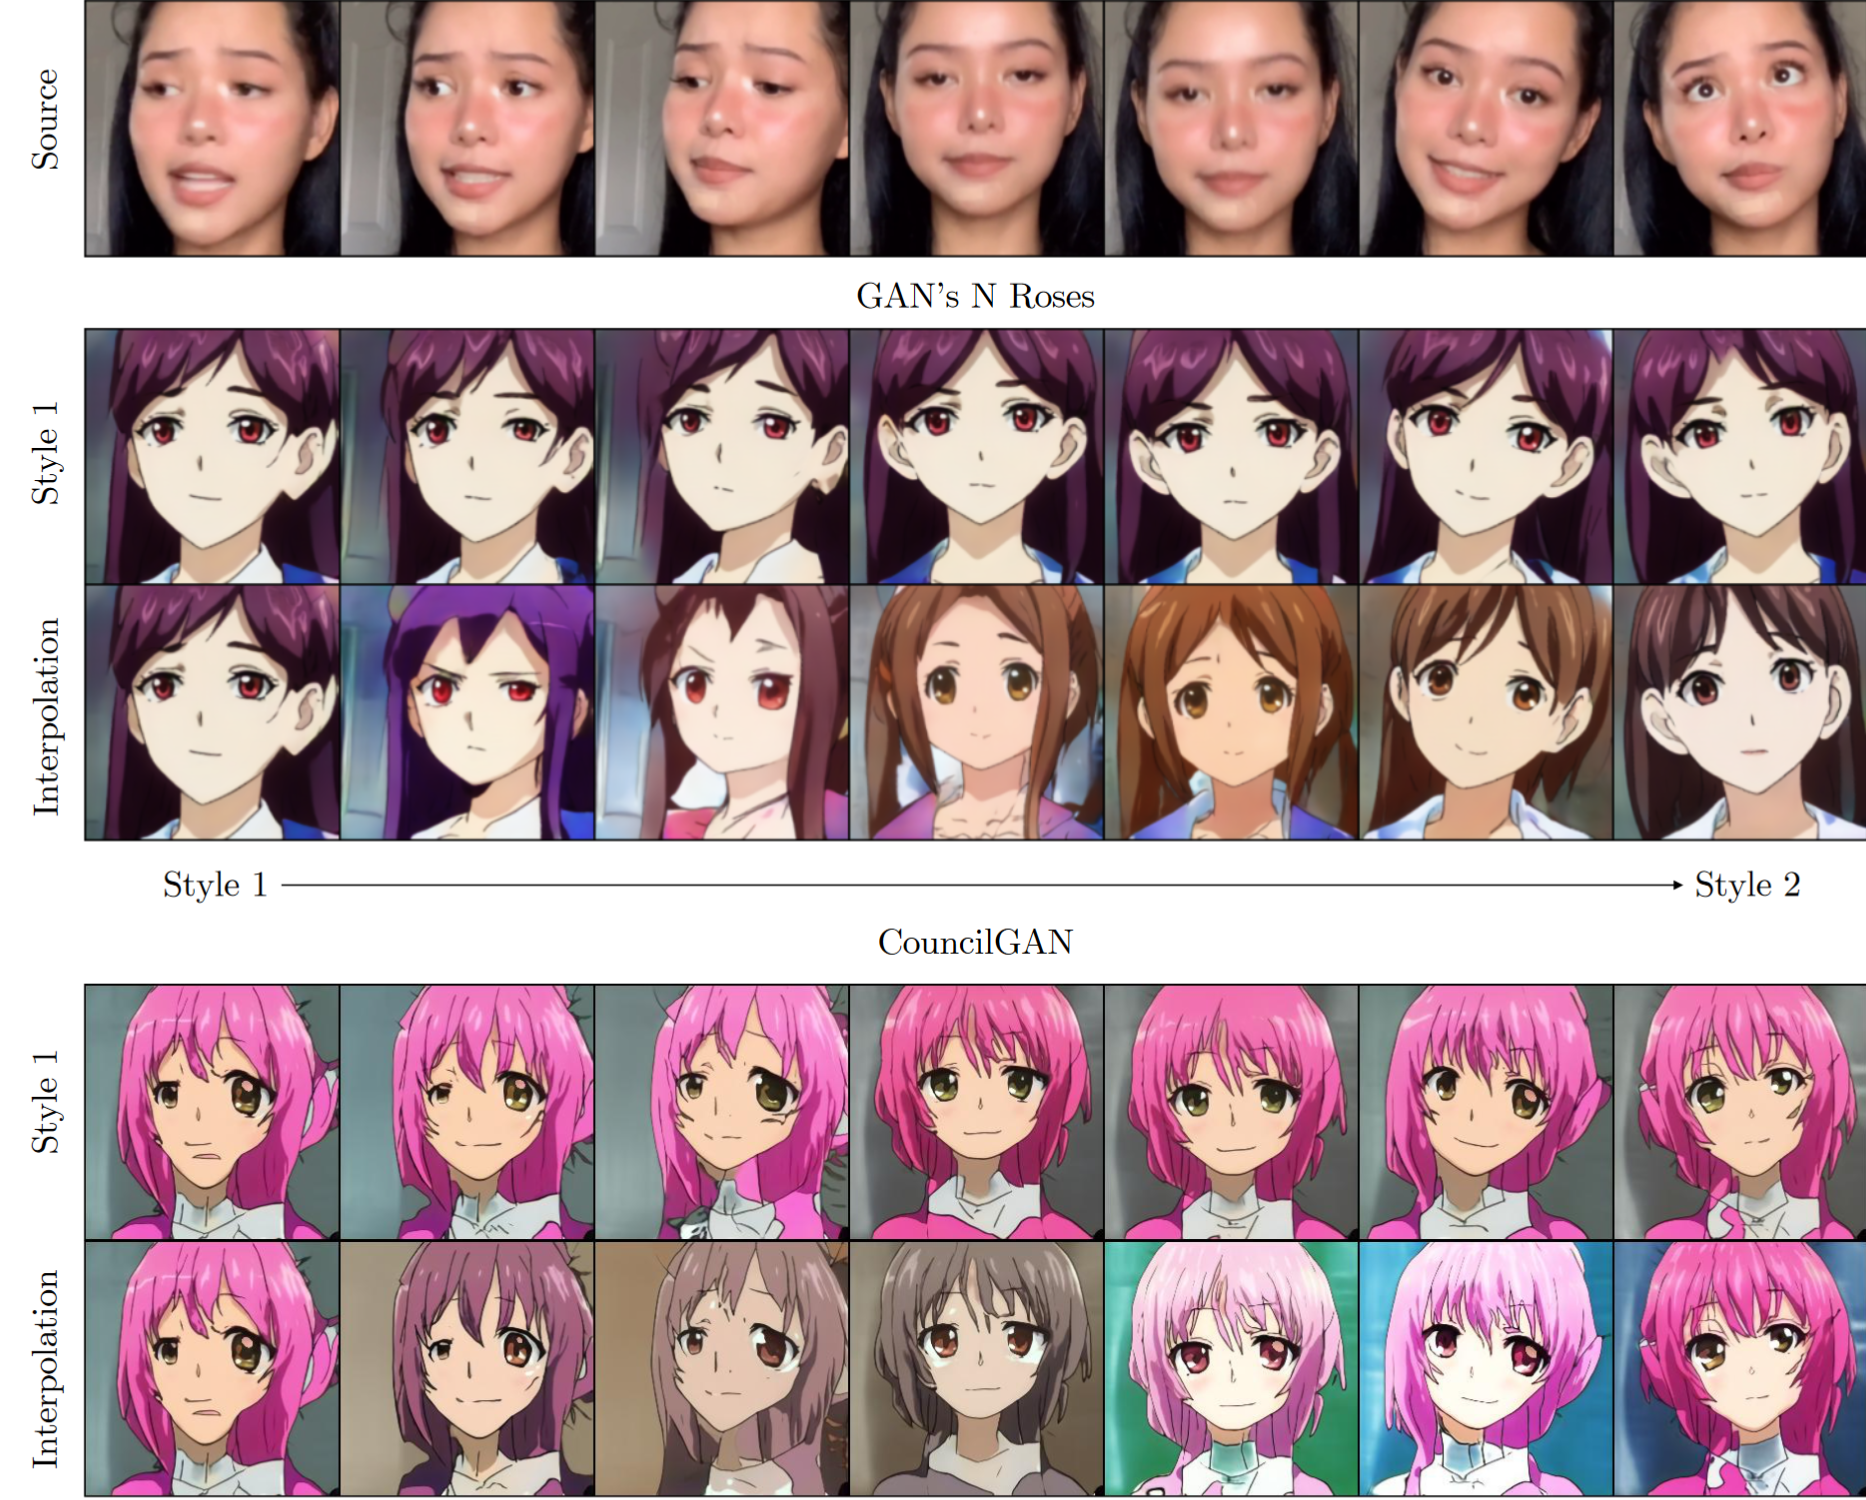
\includegraphics[width=\textwidth]{img/GNR-2.png}
    \caption{
        GANs N' Roses v.s. CouncilGAN: The {\it source} row is the input human images.
        Images under the {\it source} are generated anime characters by GNR and CouncilGAN
        \cite{chong2021gans}.
    }
\end{figure}

Ori Nizan and Ayellet Tal explains this effect in CouncilGAN as
the mismatching of geometric structures of input and training images (human image and anime image) \cite{nizan2020council}.
When AI models are trained on shojo-influenced anime datasets,
the experienced-based algorithm would detect the large eyes as a deterministic feature
of anime character,
therefore produces unreasonable eyes with weird shapes in the generated images.
As the shojo style becomes popular in the late nineteenth century,
this aesthetic idiom merged into the main stream of the manga genre \cite{takahashi2008shojo}.
This trend resulted that nearly all available training examples are some-how shojo like with large eyes, long eyelashes, and stick-like bodies.
This trend not only produces substantial similar drawing style mange and anime,
leading to a less and less diverse real world anime styles.

\begin{figure}[h]
    \includegraphics[width=\textwidth]{img/JoJo-2.png}
    \caption{
        JoJoGAN: AI generates inbetweening scenes from key scene drawing and human face expression \cite{chong2021jojogan}.
    }
\end{figure}
Furthermore, AI-generated arts are controversial,
especially in anime-related fields \cite{Sahbegovic2022anime}.
According to NihongoGamer from DoKiDoKi Drawing,
anime-drawing is generally considered as a low-paid time-consuming work \cite{NihongoGamer2022drawing}.
As Yazuki Wolf mentioned during the interview,
AI saves substantial time in anime production by taking over inbetweening.
In this case, artists can only draw the key frames and let the AI fill in between with different angles of the same scene and the characters as shown in Figure 6.

However, critics toward AI drawing is mainly focused on two factors:
the limited market of drawing and plagiarism \cite{Sahbegovic2022anime}.
Thomas Lamarre states that 
``anime technosocial mode of existence has emerged as an internal limit on the
distributive force of television, appearing where television folds back on itself
in an assembling of polarized tendencies that at once affects and follows from
specific kinds of content and audiences as well as platforms and infrastructures \cite{Lamarre2018Anime}.''
Also argued by Sahbegovic,
people are trying to sell AI-generated artworks in an already overcrowded market
with loads of gifted artists \cite{Sahbegovic2022anime}.
Secondly, Sahbegovic mentions that generative AI models amplify plagiarism in two ways:
\begin{enumerate}
    \item finishing sketches by AI and publish the work before the original author
    \item generating images with pieces from other artworks without acknowledgement.
\end{enumerate}
   
The first type of access to plagiarism is due to LDMs' fantastic ability of semantic 
synthesis with given conditional reference.
Personally, I think this issue could be resolved by not exposing unfinished drawing drafts to the public.
And the second type plagiarism is caused by the nature of machine learning:
taking information from the existing dataset and produce a combination of these old data.
In this case, I argue that better data-preprocessing and selection could contribute to this to a large extent.
\begin{figure}[h]
     \centering
     \begin{subfigure}[b]{0.49\textwidth}
         \centering
         \includegraphics[width=0.7\textwidth]{img/LDM-2.png}
         \caption{
            AI-drawing (left) generated from sketch v.s. 
            author's finished the drawing (right) \cite{Sahbegovic2022anime}.
        }
     \end{subfigure}
     \hfill
     \begin{subfigure}[b]{0.49\textwidth}
         \centering
         \includegraphics[width=\textwidth]{img/LDM-3.png}
         \caption{LDM completion of sketch of landscape scene \cite{Rombach2022High}.}
     \end{subfigure}
     \hfill
     \caption{Comparison of sketch to final generated image.}
\end{figure}
